% !TeX spellcheck = it_IT
\newpage
\section{Introduzione}
Il corso prevede di affrontare assieme due degli ambiti più importanti al giorno d'oggi: \textbf{trasformazione digitale} e \textbf{transizione verde}.
\subsection{Trasformazione digitale}
Con il tempo c'è stata un'evoluzione delle reti di comunicazioni esponenziale grazie alla diffusione di reti pervasive a banda ultra-larga e a basso costo. Inoltre, a causa della diffusione di servizi digitali per la condivisione di dati multimediali ad alta risoluzione, c'è una produzione, un trasferimento ed un consumo di una mole di dati sempre maggiore.
\begin{center}
	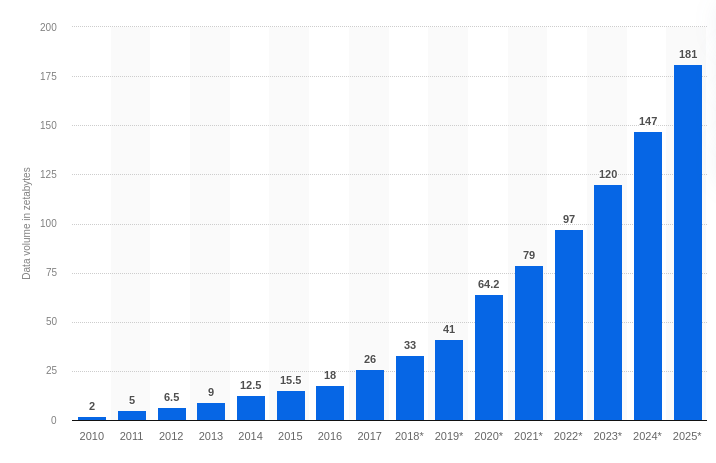
\includegraphics[scale=0.5]{data_creation.png}
\end{center}
Numerosi sono i programmi di sviluppo nazionali ed europei mirati proprio alla trasformazione digitale, favoriti anche dalla pandemia di Covid-19. Un esempio classico è il \href{https://www.mimit.gov.it/it/pnrr/piano}{PNRR}:
\begin{center}
	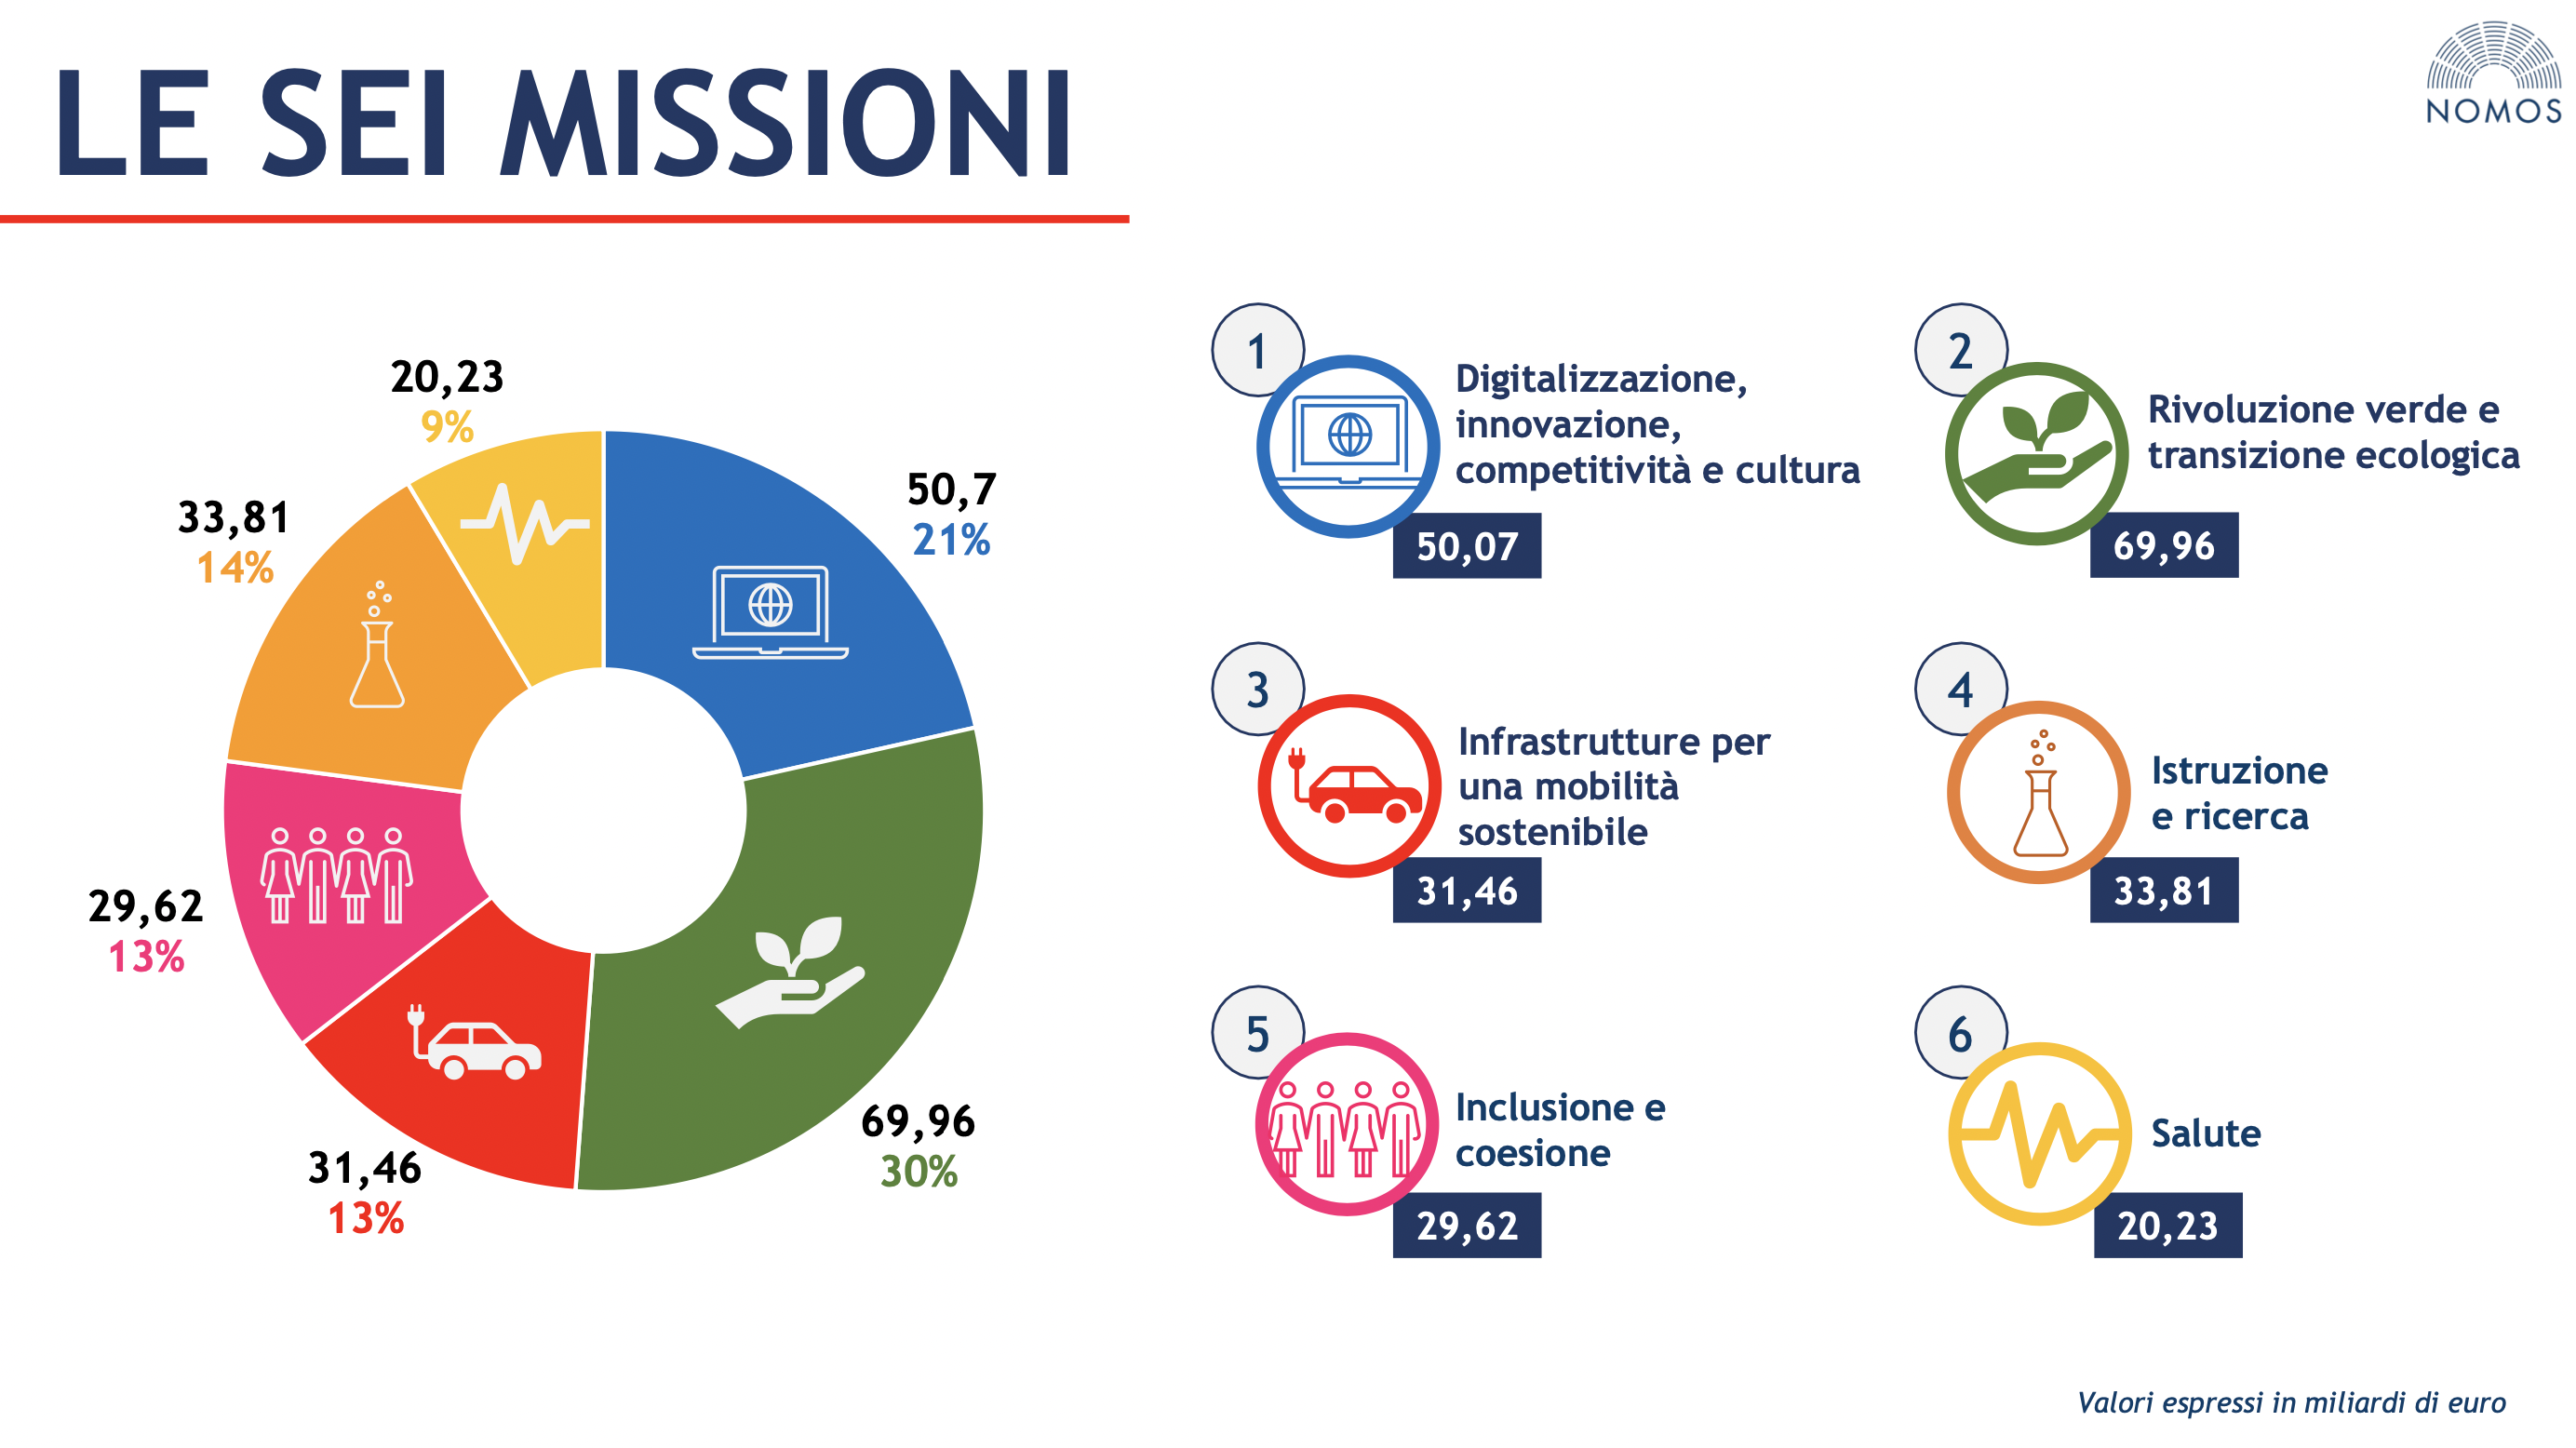
\includegraphics[scale=0.2]{missioni-pnrr.png}
\end{center}

\newpage
\subsection{Consumo energetico}
Il consumo energetico da parte del settore ICT è ad oggi il $5\%$ della domanda mondiale ed è previsto che superi il $20\%$ nel 2030. La produzione di $CO_2$ del settore è pari al $2\%$, quanto quella degli aerei.
\begin{center}
	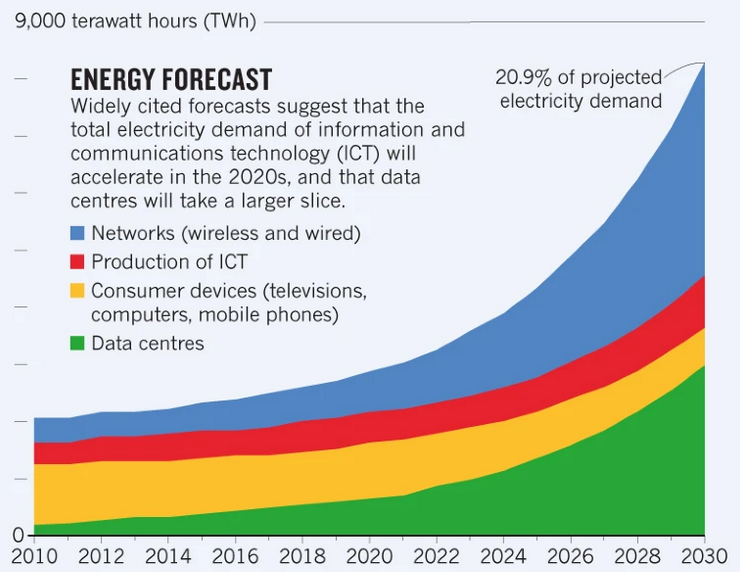
\includegraphics[scale=0.3]{energy_consumption.png}
\end{center}

\subsection{Dennard scaling}
È una legge empirica che sostiene che riducendo la dimensione dei transistor, il rapporto tra potenza e superficie ($watt/cm^2$) rimane costante.


\subsection{E-waste}
La continua emissione di dispositivi guasti o passati di moda contribuisce ad alimentare i rifiuti di apparecchiature elettriche ed elettroniche (RAEE). \\
Questi 50 milioni di rifiuti finiscono nei paesi in via di sviluppo dove non vengono smaltite correttamente (danno per l'ambiente e non-biodegradabilità).

\subsection{Paris Agreement}
Un accordo legalmente vincolante per mantenere il riscaldamento globale ben al di sotto dei $2°C$ e idealmente sotto $1.5°C$ basato sui seguenti principi:
\begin{itemize}
	\item \textit{Obiettivo a lungo termine}, con piani quinquennali
	\item \textit{Contributi} dei vari paesi
	\item \textit{Ambizione}
	\item \textit{Trasparenza} sui dati
	\item \textit{Solidarietà} dei paesi più sviluppati verso quelli in via di sviluppo
\end{itemize}
Per rispettare l'accordo ogni europeo dovrebbe ridurre le emissioni da 10 a 2 tonnellate di $CO_2$.

\subsubsection{Aziende}
Le aziende informatiche sono interessate al green computing per:
\begin{itemize}
	\item Ridurre i costi di gestione ed aumentare gli utili
	\item Migliorare la reputazione aziendale verso il personale
	\item Greenwashing
	\item Realizzare una trasformazione energetica
\end{itemize}